\section{PI Force Controller}
In this section, the central illustration for the PI Force Controller is depicted. On the left, the figure showcases the arm's movement, where the oval shape symbolizes the patient's body and the lines provide a basic representation of the arm (see Figure \ref{fig:armsimplification}). The movement starts at the green dot and concludes at the red dot. The large blue dot indicates the desired position, while the series of smaller blue dots trace the arm's trajectory. On the right, the graph presents the forces (in Newtons) over time (in Seconds), detailing the forces across the three axes.

\begin{figure}[h!] 
    \centering
    \begin{subfigure}[b]{0.45\linewidth}
        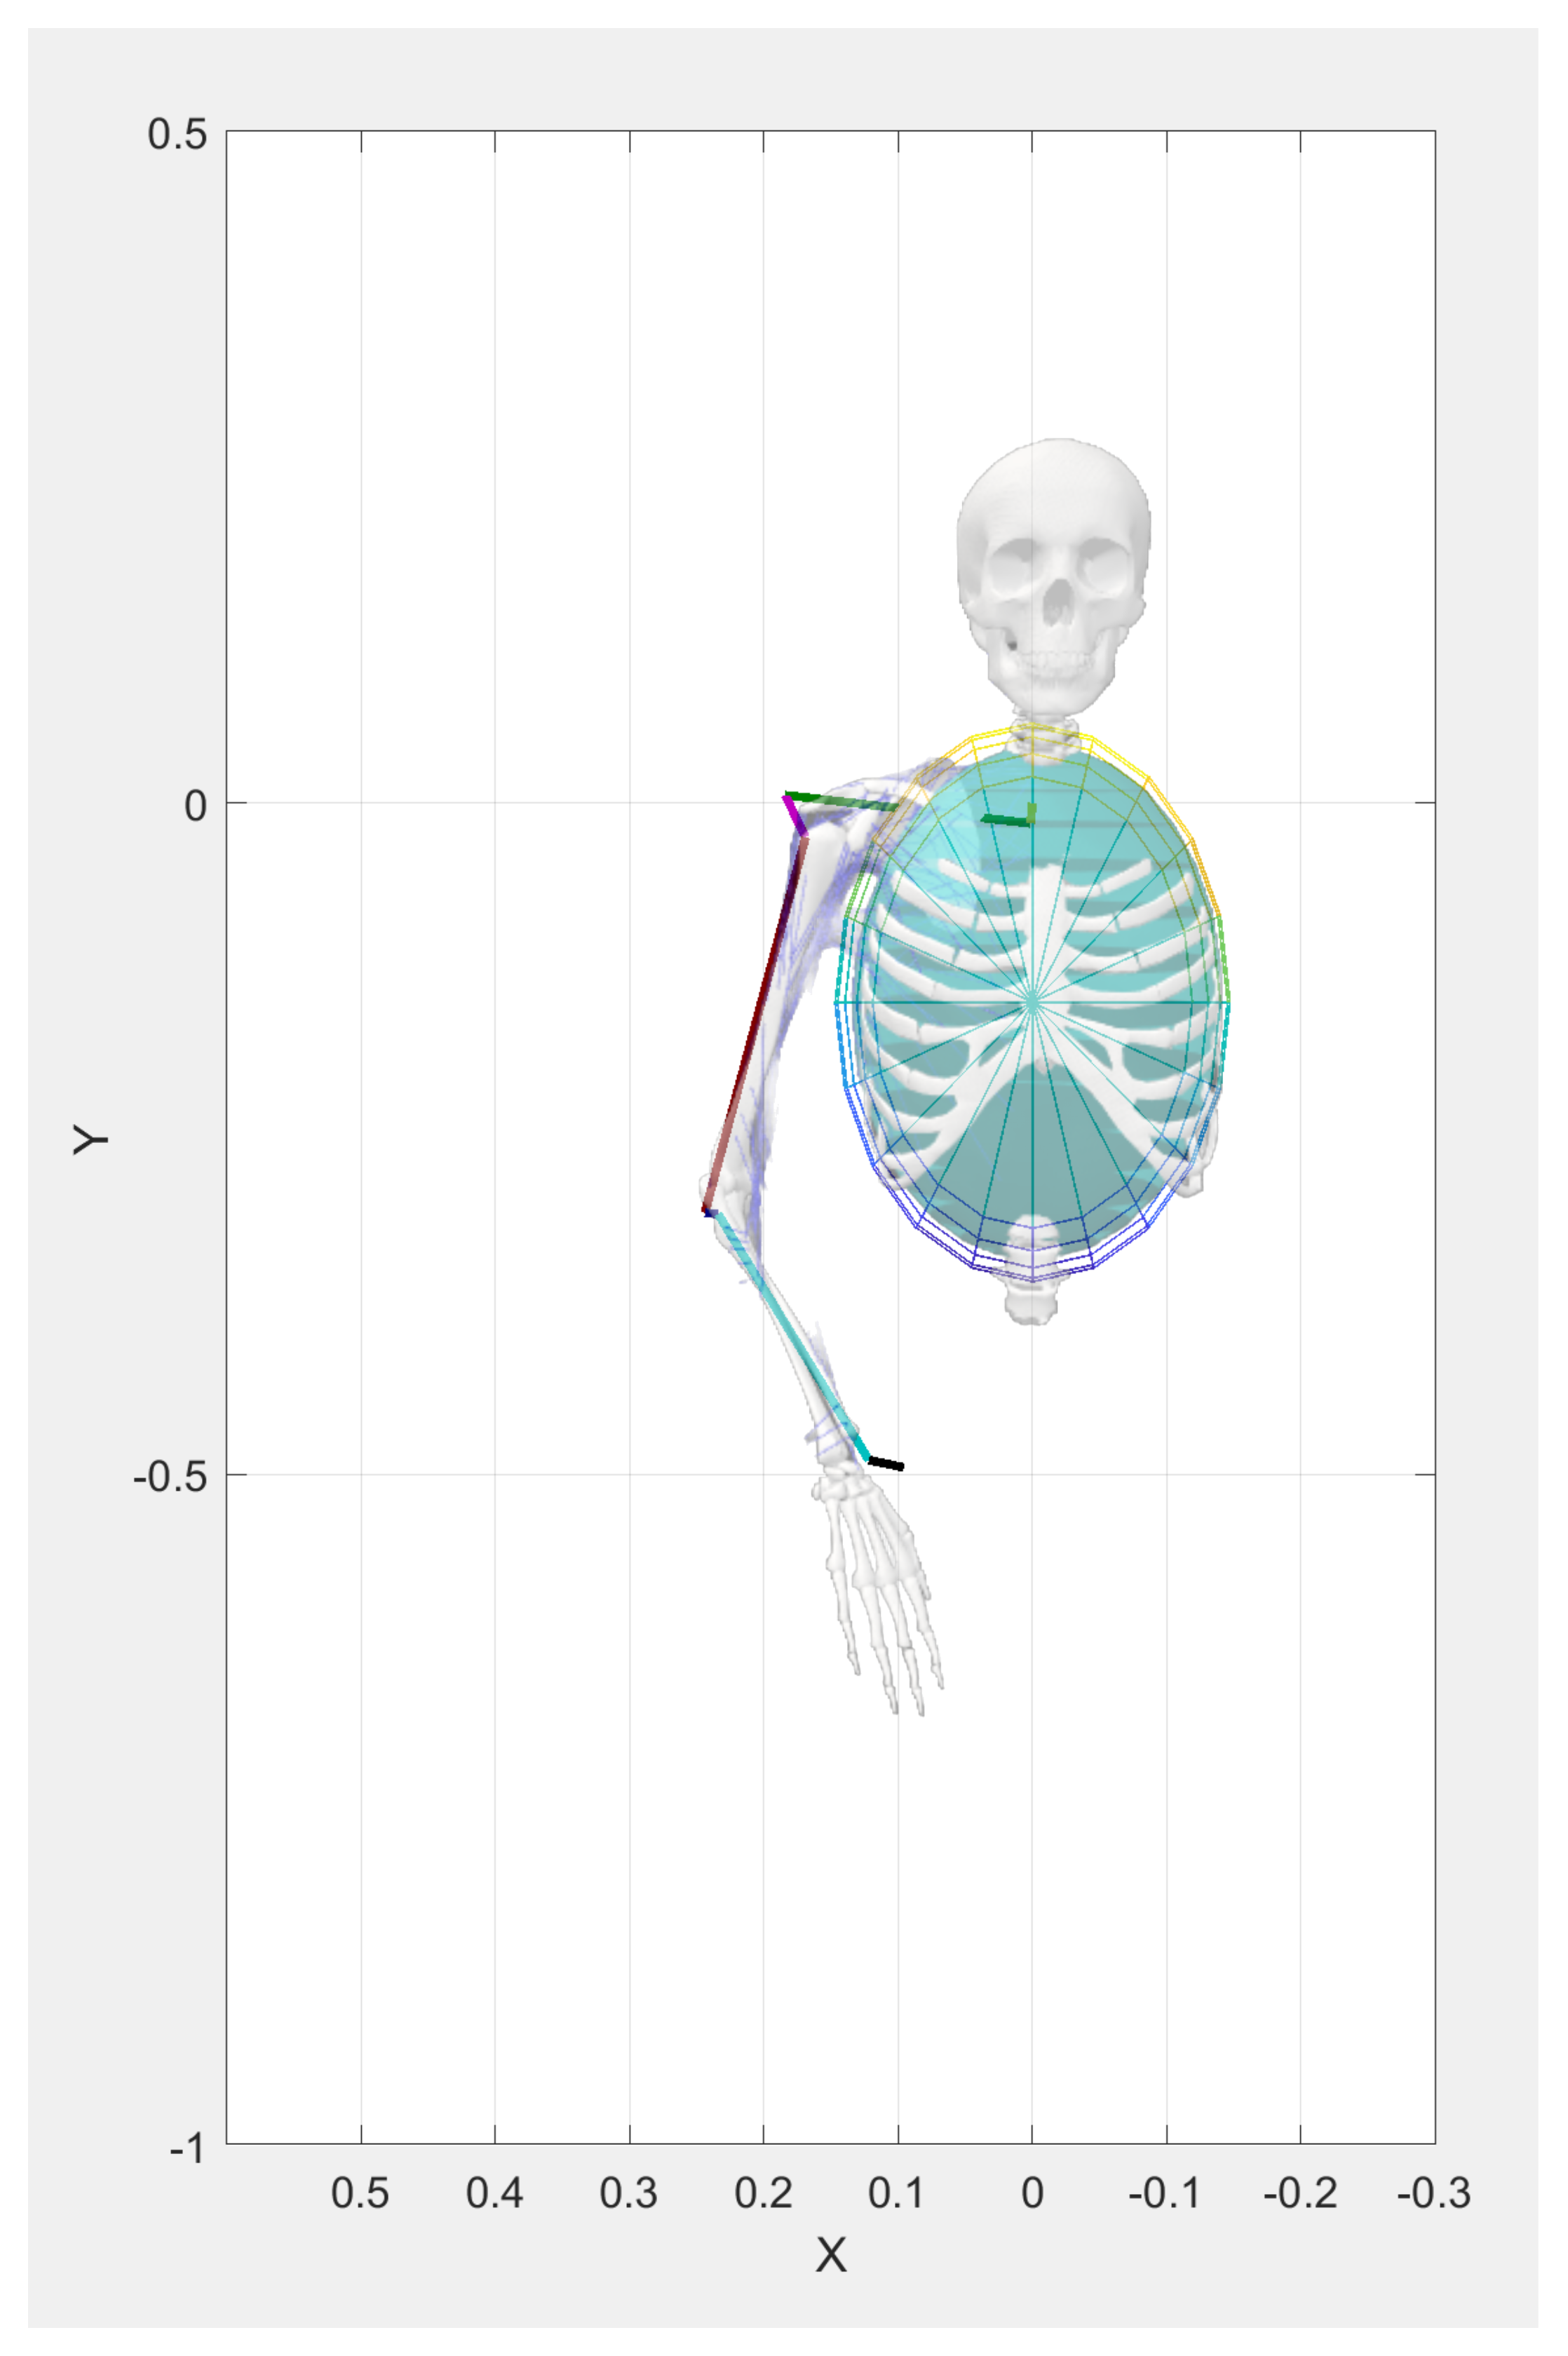
\includegraphics[width=0.8\textwidth]{Pictures/Results/armbackground.png}
        \caption{Arm Simplification MATLAB vs Open SIM}
        \label{fig:armsimplification}
    \end{subfigure}
    \hfill
    %\vspace{1cm} % Adjust the space between the figures as needed
    \begin{subfigure}[b]{0.45\linewidth}            
        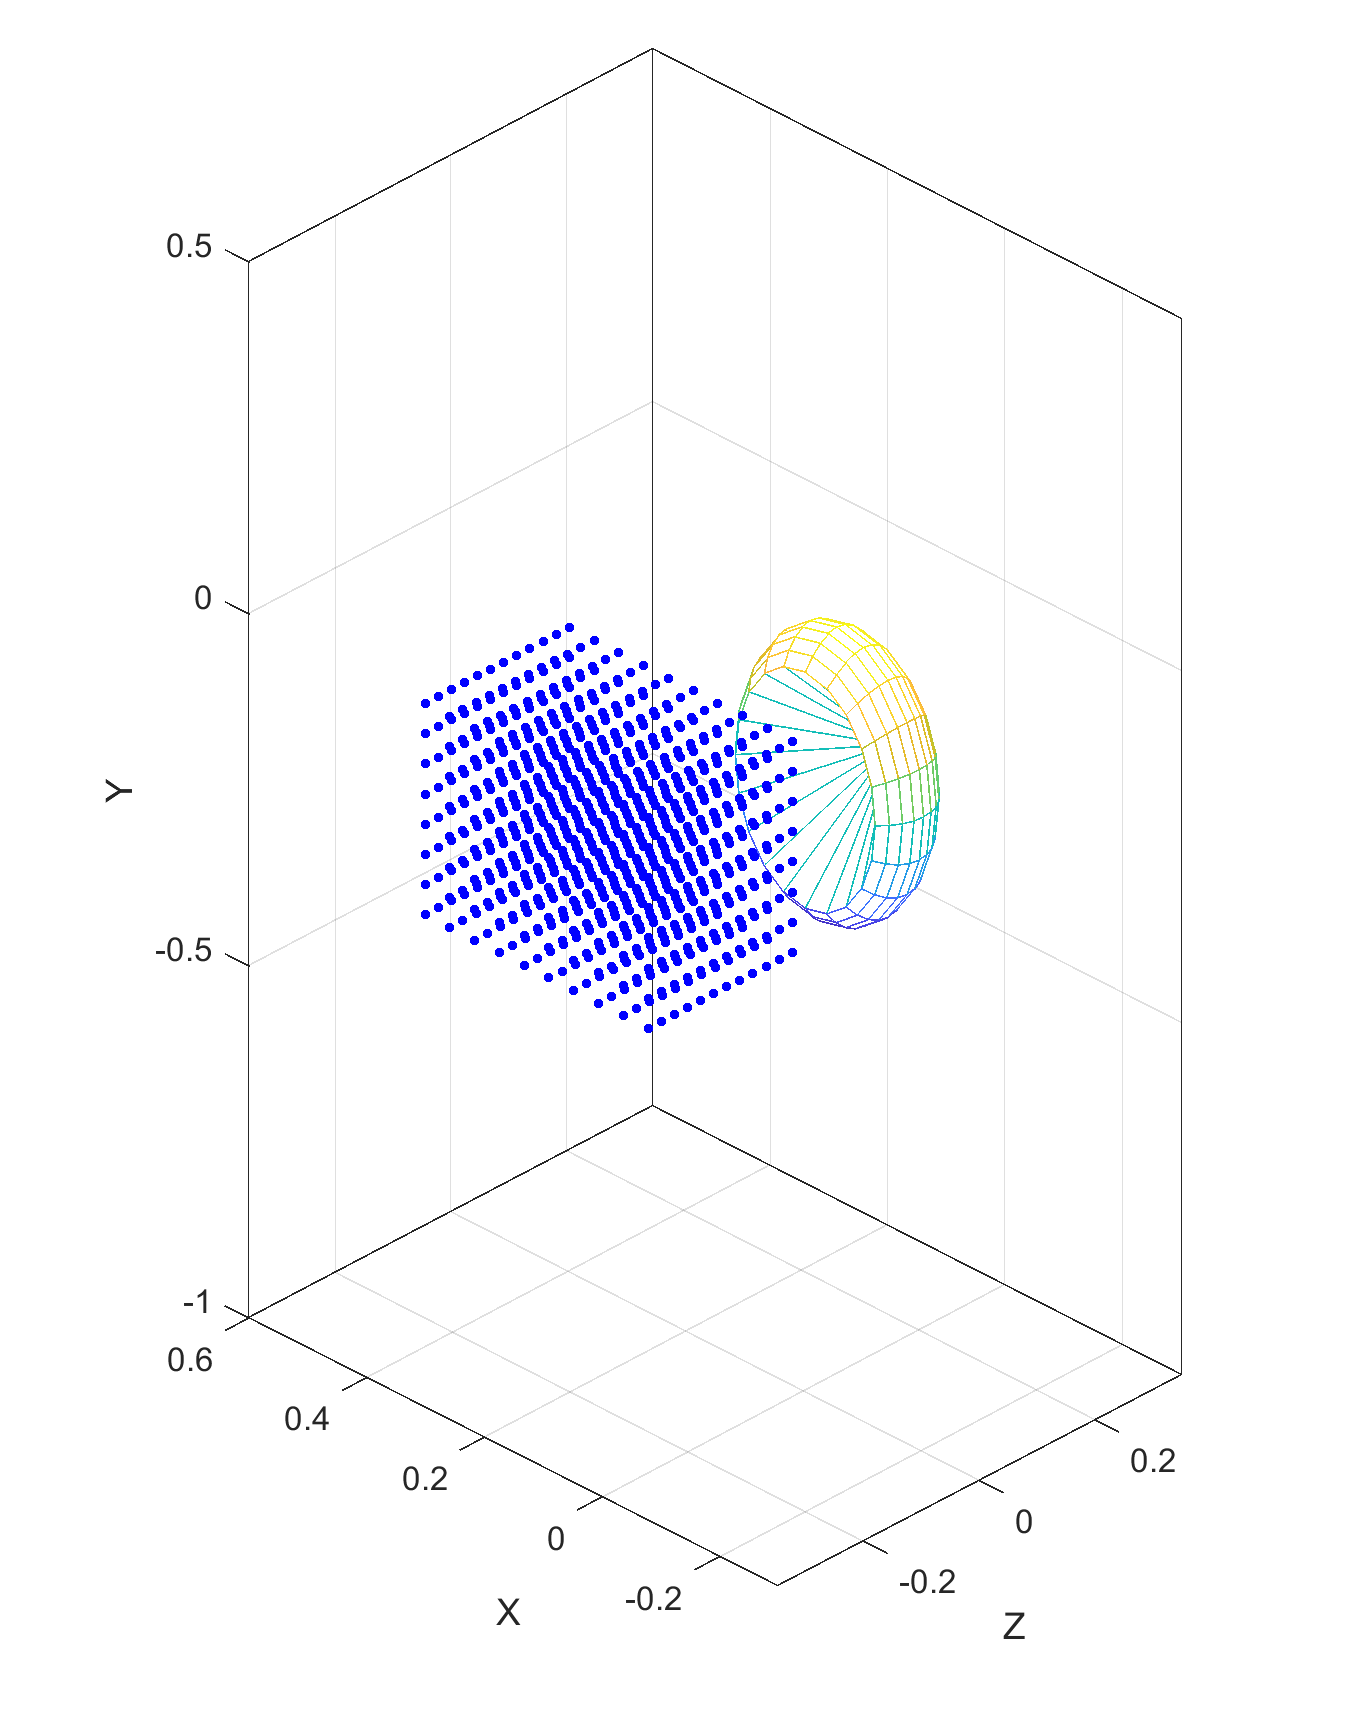
\includegraphics[width=0.9\textwidth]{Pictures/Results/960points.png}
        \caption{960 reference point used for the PI Controller}
        \label{fig:960}
    \end{subfigure}
\end{figure}


The PI controller was successfully implemented across 960 points (see Figure \ref{fig:960}), and the corresponding forces were computed based on a specified muscle dictionary. However, only 64 of this points were as data to calculate the torques for the models.

The two subsequent GIFs (\ref{gif:PICONTROLLER1}, \ref{gif:PICONTROLLER2}), best viewed in Adobe Acrobat, illustrate the OpenSim movement under the PI Controller with and without neural excitation. One demonstrates the transition from a static to the desired position, while the other showcases maintaining the position during triceps stimulation

\subsection{PI vs PID Controller}

In the evaluation process for optimizing PI parameters, it was observed that integrating the derivative term (D) of the PID controller did not yield significant improvements in performance. As a result, the simpler PI model was adopted. A comparison between PI and PID performances is provided in the accompanying image. For the PI model, the constants utilized were Kp = 2000 and Ki = 100.

\begin{figure}[h!] 
    \centering
    \begin{subfigure}[b]{0.8\linewidth}
       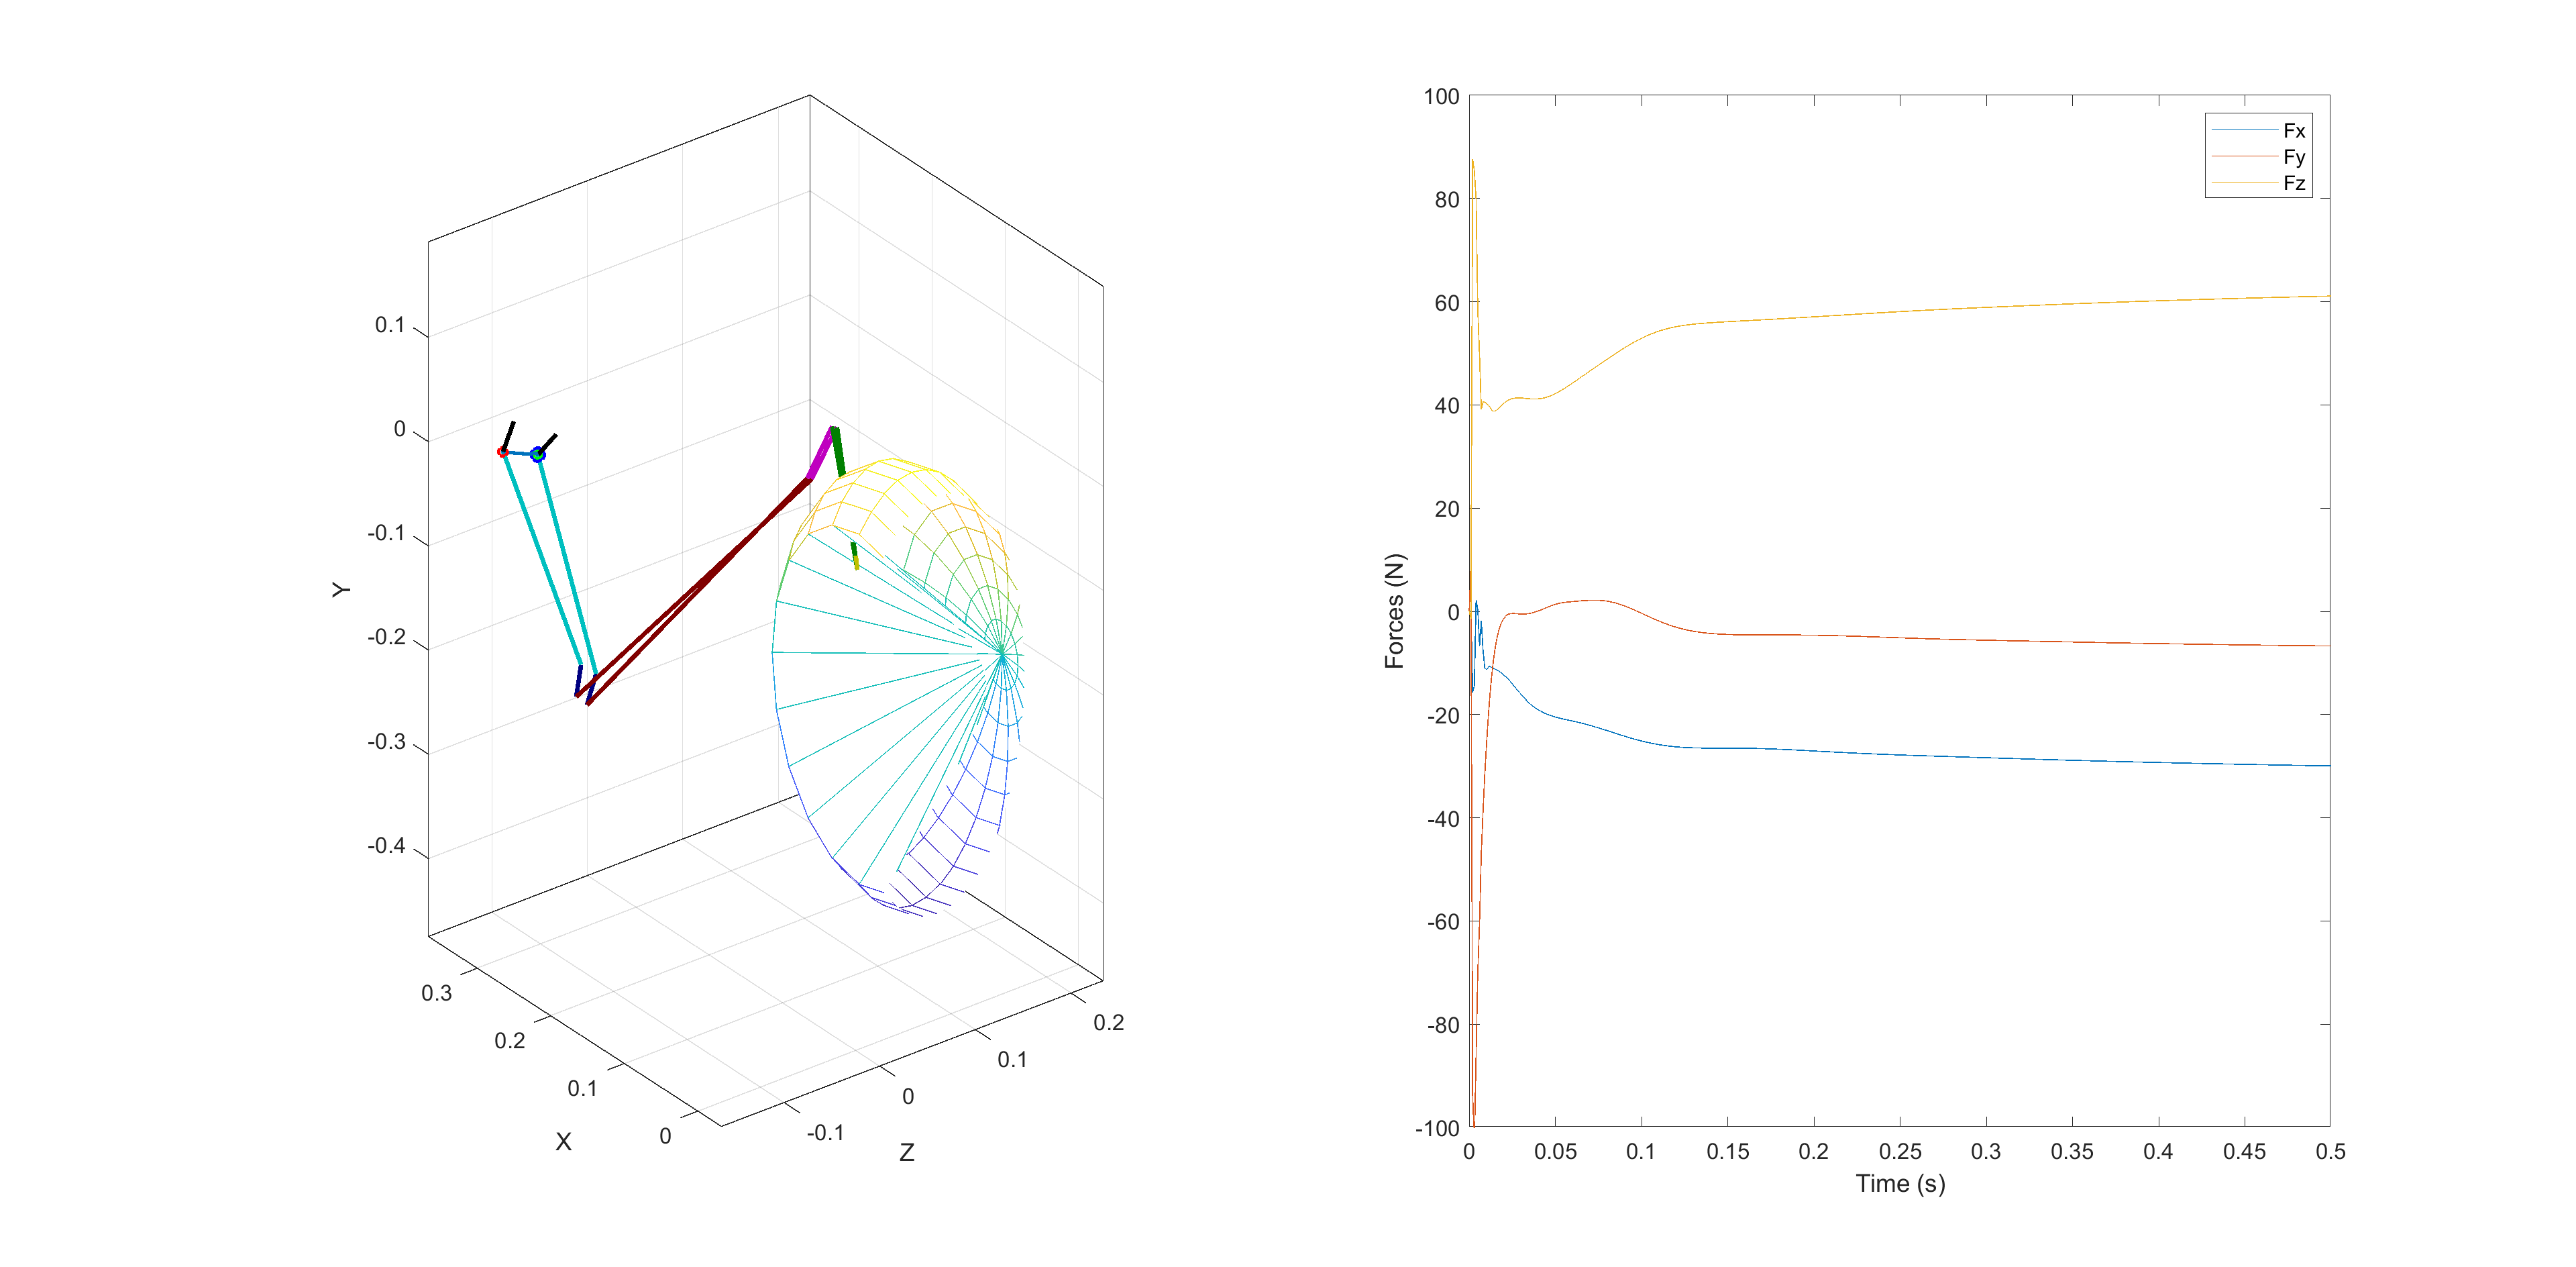
\includegraphics[width=\linewidth]{Pictures/Results/PIDController_NeuralExcitation.png}
        \caption{PID Controller.}
    \end{subfigure}

    \vspace{1cm} % Adjust the space between the figures as needed
    \begin{subfigure}[b]{0.8\linewidth}            
        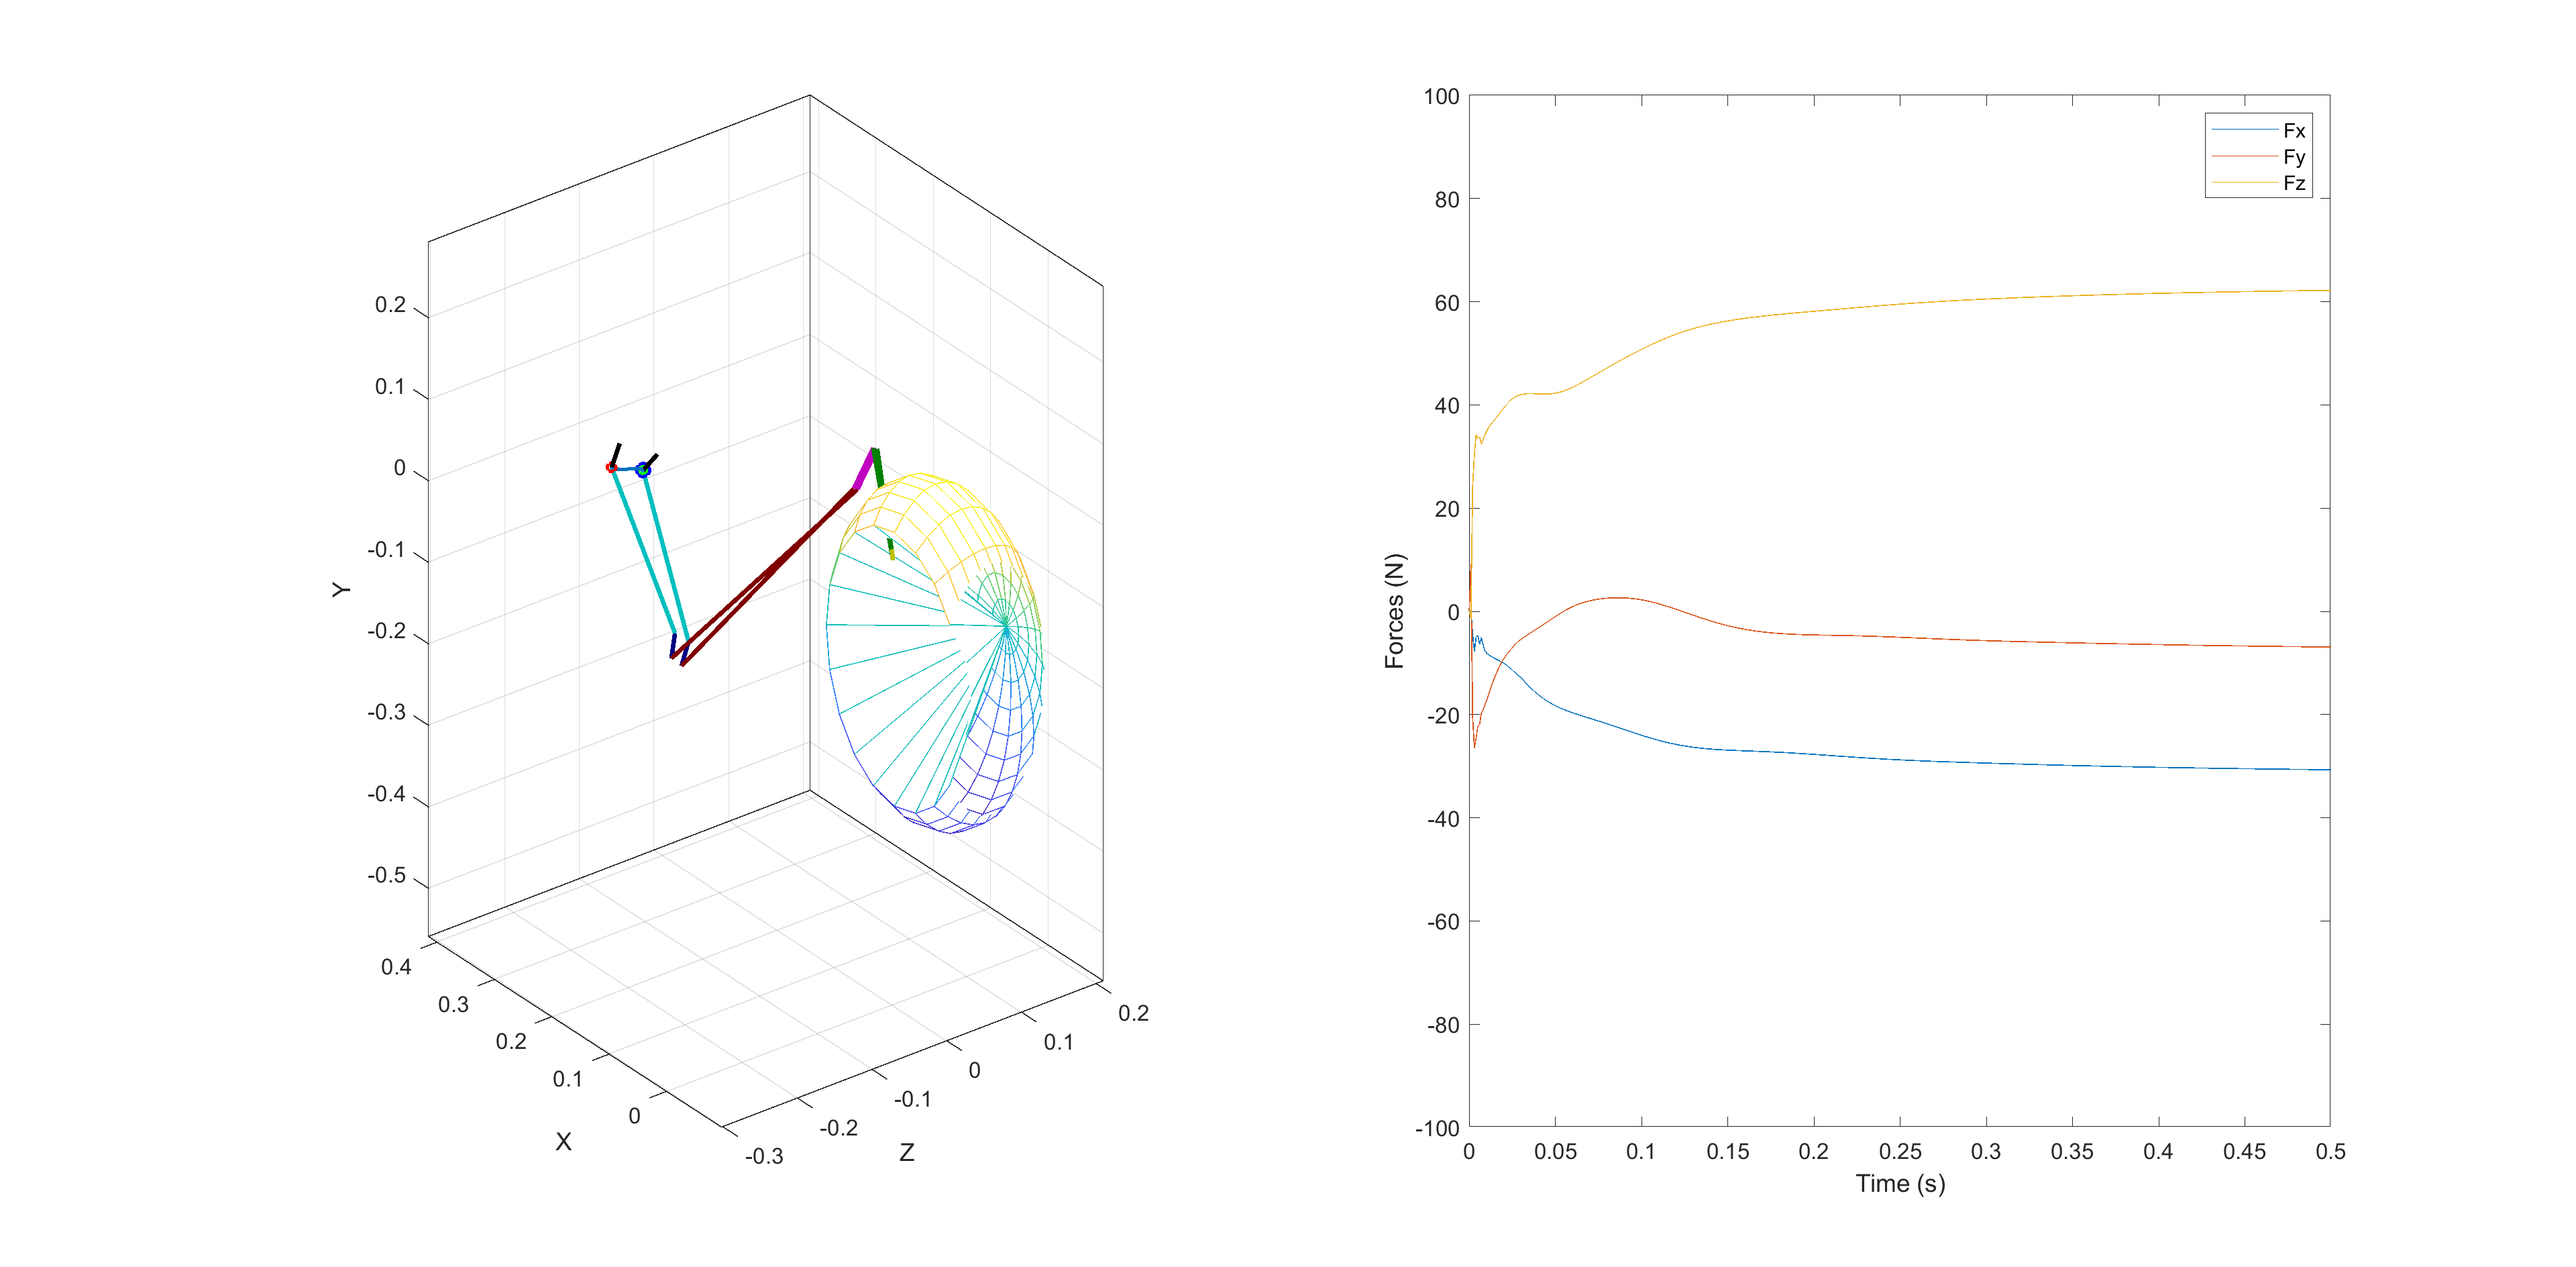
\includegraphics[width=\linewidth]{Pictures/Results/PIController_NeuralExcitation.png}
        \caption{PI Controller.}
    \end{subfigure}

    \caption{Holding Static Position with One Muscle Excitation.}

\end{figure}

\subsection{1s vs 3s Duration for Simulations Without Neural Excitation}

Initially, simulations were conducted over a 3-second duration. However, upon iterative testing, it was discerned that a duration of 1 second was sufficient. The introduction of arm support reinforced this observation, as a marked reduction in oscillations was noted, leading to faster arm stabilization. A comparative analysis between scenarios with and without arm support is explored in the subsequent section.

\begin{figure}[h!] 
    \centering
    \begin{subfigure}[b]{0.8\linewidth}
       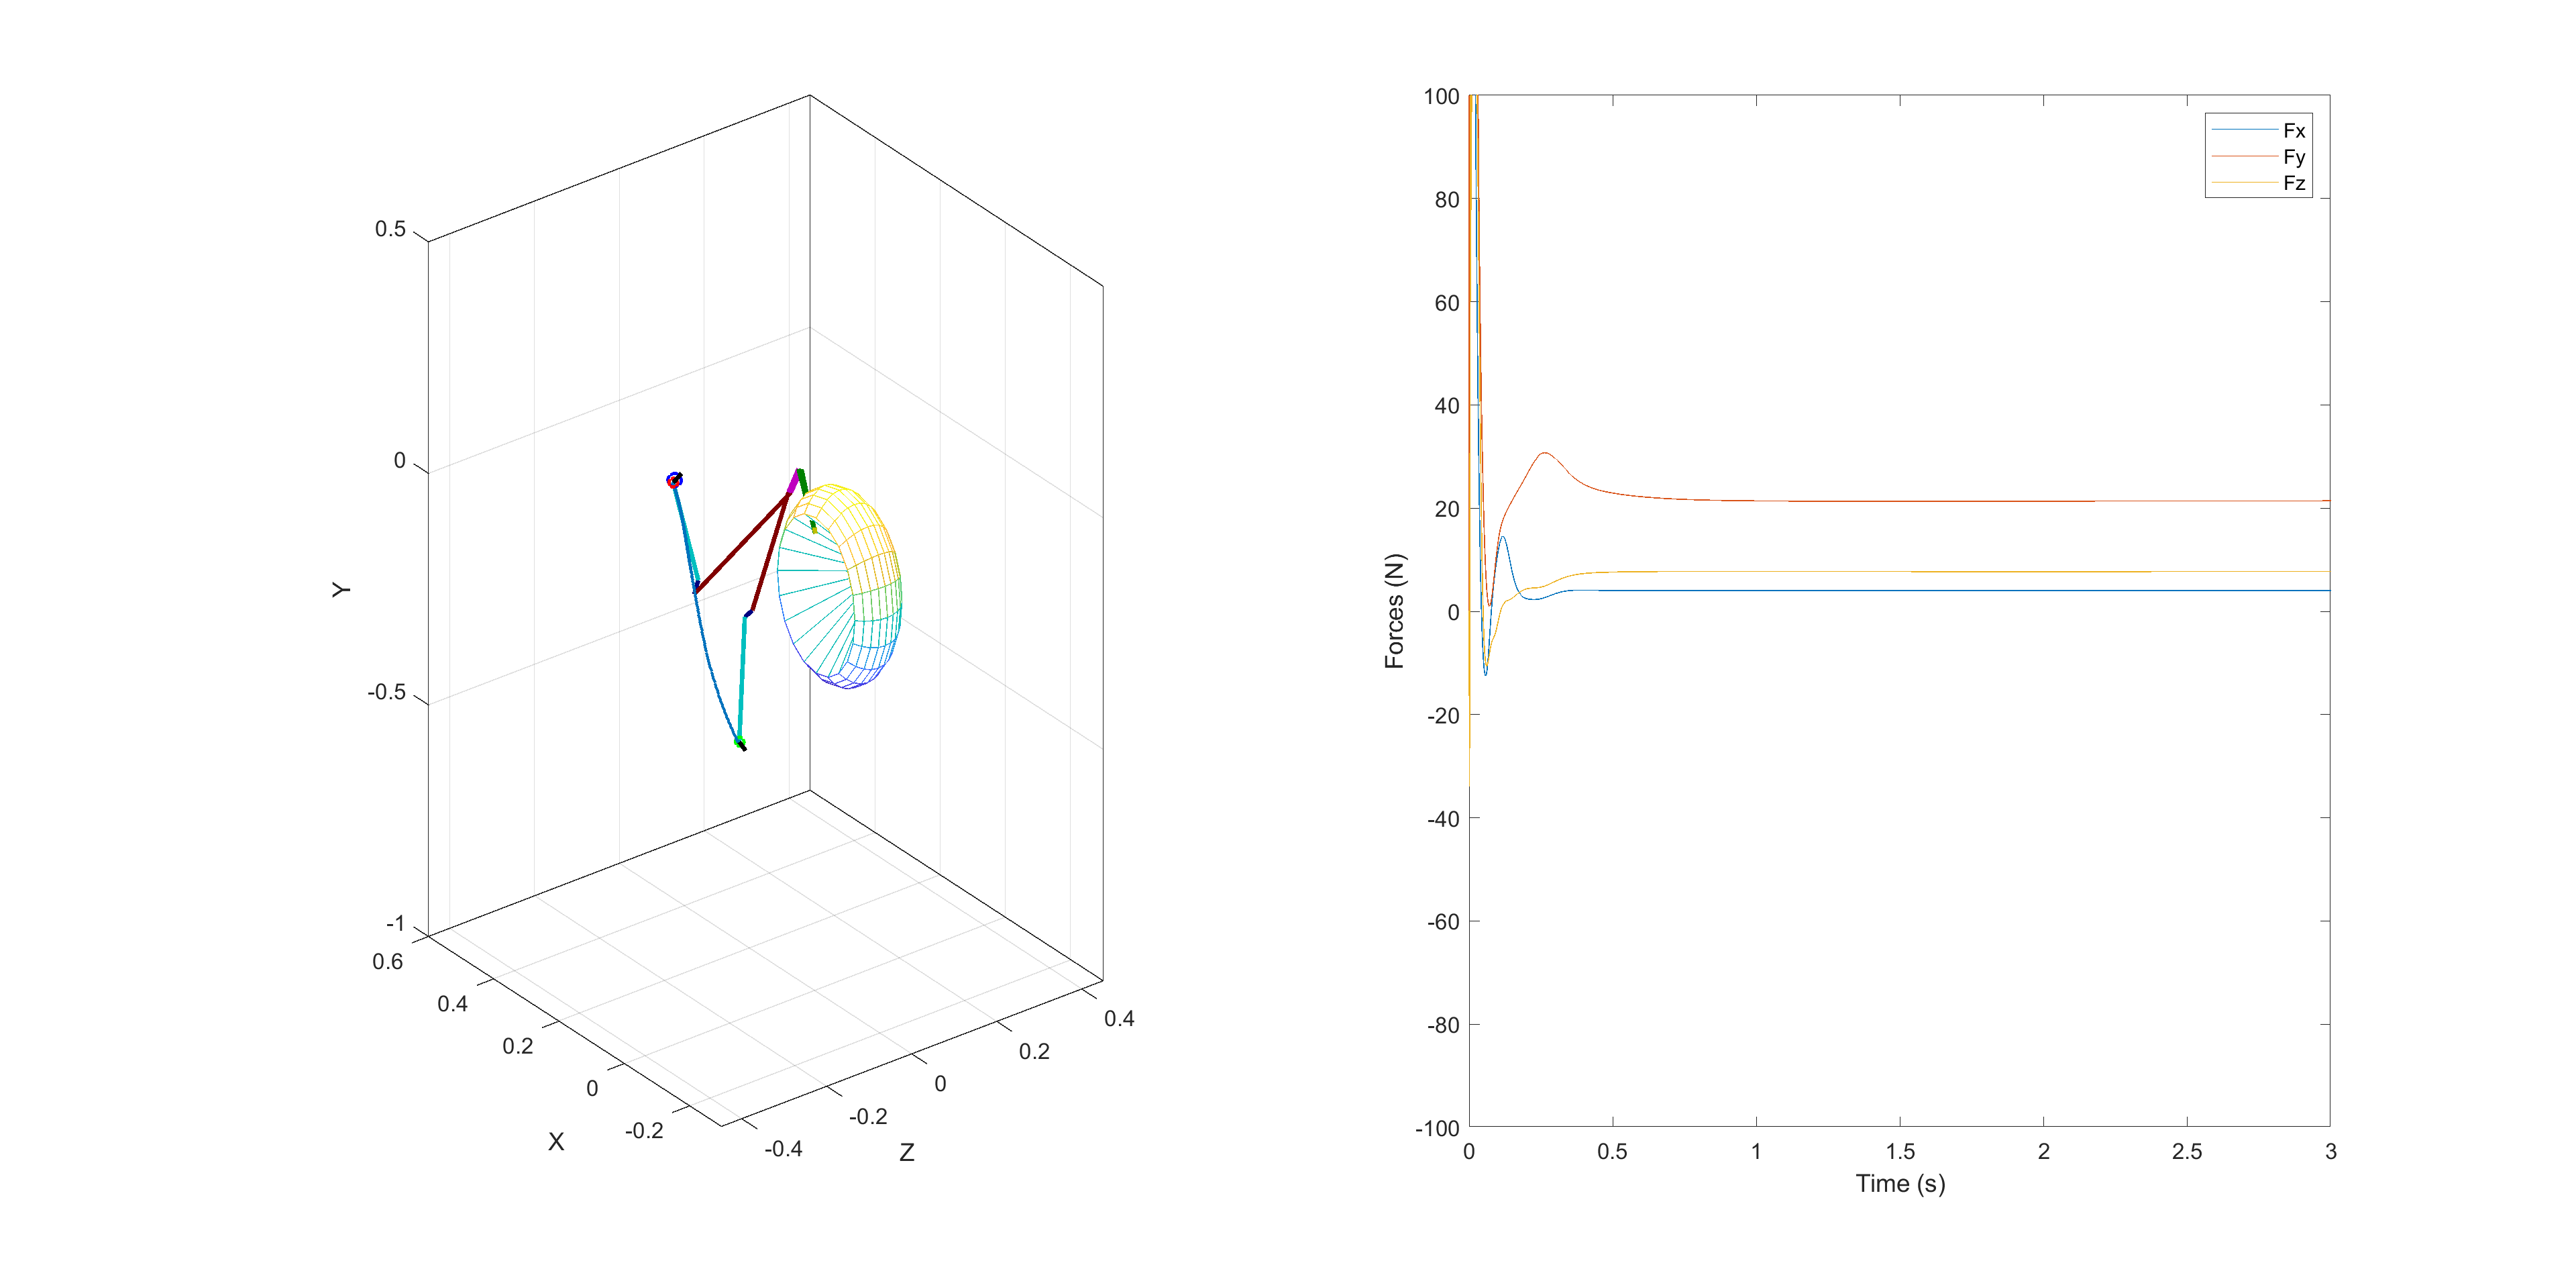
\includegraphics[width=\linewidth]{Pictures/Results/3s_NoNeuralExcitation.png}
        \caption{PI Controller 3 seconds Simulation.}
    \end{subfigure}

    \vspace{1cm} % Adjust the space between the figures as needed
    \begin{subfigure}[b]{0.8\linewidth}            
        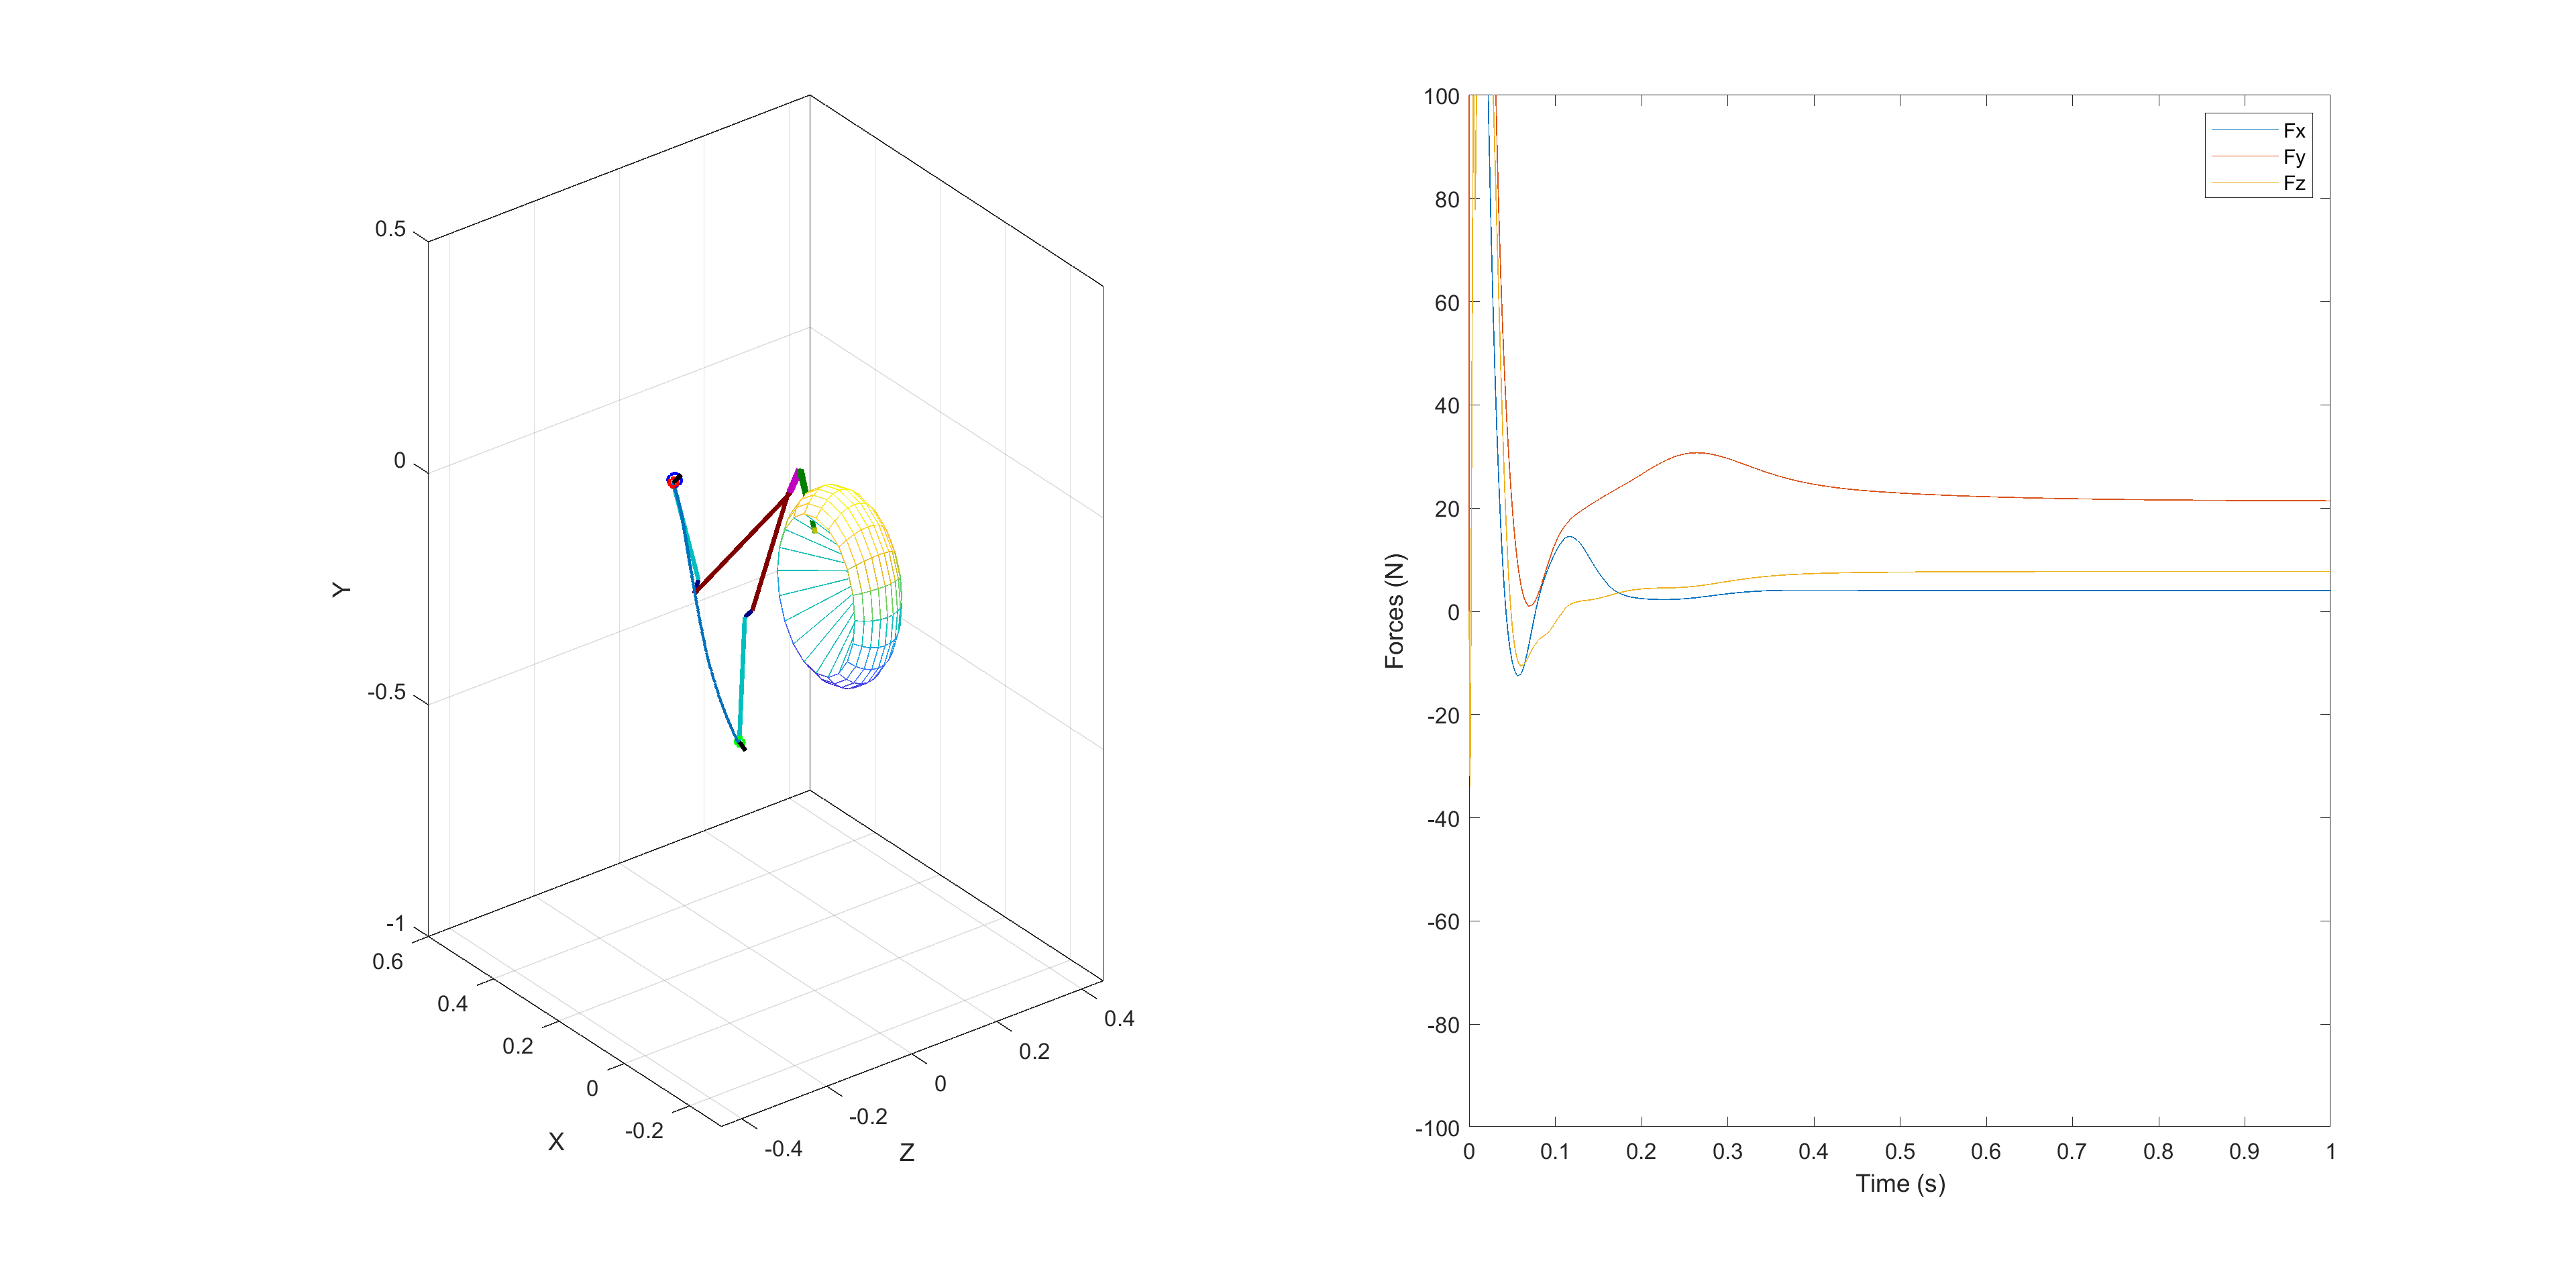
\includegraphics[width=\linewidth]{Pictures/Results/1s_NoNeuralExcitation.png}
        \caption{PI Controller 1 second Simulation.}
    \end{subfigure}

    \caption{PI Controller from Equilibrium Position to Static Position with No Muscles Excitation.}

\end{figure}

\begin{figure}[h!]
    \centering
    \animategraphics[timeline=timeline.txt,autoplay,loop,width=0.75\textwidth]{12}{Pictures/Results/NoExct/frame_}{11}{45}
    \caption{PI Controller No Excitation from Equilibrium Position. Open in Adobe Acrobat to see gif movement.}
    \label{gif:PICONTROLLER2}

\end{figure}

\begin{figure}[h]
    \centering
    \animategraphics[timeline=timeline.txt,autoplay,loop,width=0.75\textwidth]{12}{Pictures/Results/TricepsExct/frame_}{0}{34}
    \caption{PI Controller maintaining Static Position with Triceps Excitation. Open in Adobe Acrobat to see gif movement.}
    \label{gif:PICONTROLLER1}
\end{figure}

\subsection{Support vs Non-Support}
Inspired on the work done in the research \cite{HSAC},\cite{QSC} and \cite{RTS} an arm support component was integrated into the PI controller to simulate the robotic arm that held the patient's arm as they suffered from spinal cord injury that did not allow them to lift their arm. In the scope a project, an arm support is added to mimic the common scenario observed in stroke survivors, where they leverage their own strength to support and stabilize their affected arm during rehabilitation exercises. The inclusion of this arm support component in the simulation is pivotal, as it offers a more realistic representation of the rehabilitation process. By accounting for the patient's inherent capability to self-support, the simulation ensures that the outcomes align closely with real-world scenarios, paving the way for more tailored and effective rehabilitation strategies. In the code of Matlab this arm support mechanism acts provides an additional force to guide the hand toward a desired position and maintaining stability by mitigating rapid or undesirable movements. 

As seen in the Figures below the arm support reduces oscillation improving the stability of the control. On the top image the figure shows the simulation to find the equivalent force without arm support and on the bottom figure the simulation with arm support. Figure \ref{fig:PINoExcitation} presents the case when no neural excitation is provided and Figure \ref{fig:PIExcitation} when Neural Excitation is given for one muscle.

\begin{figure}[h!] 
    \centering
    \begin{subfigure}[b]{0.45\linewidth}
       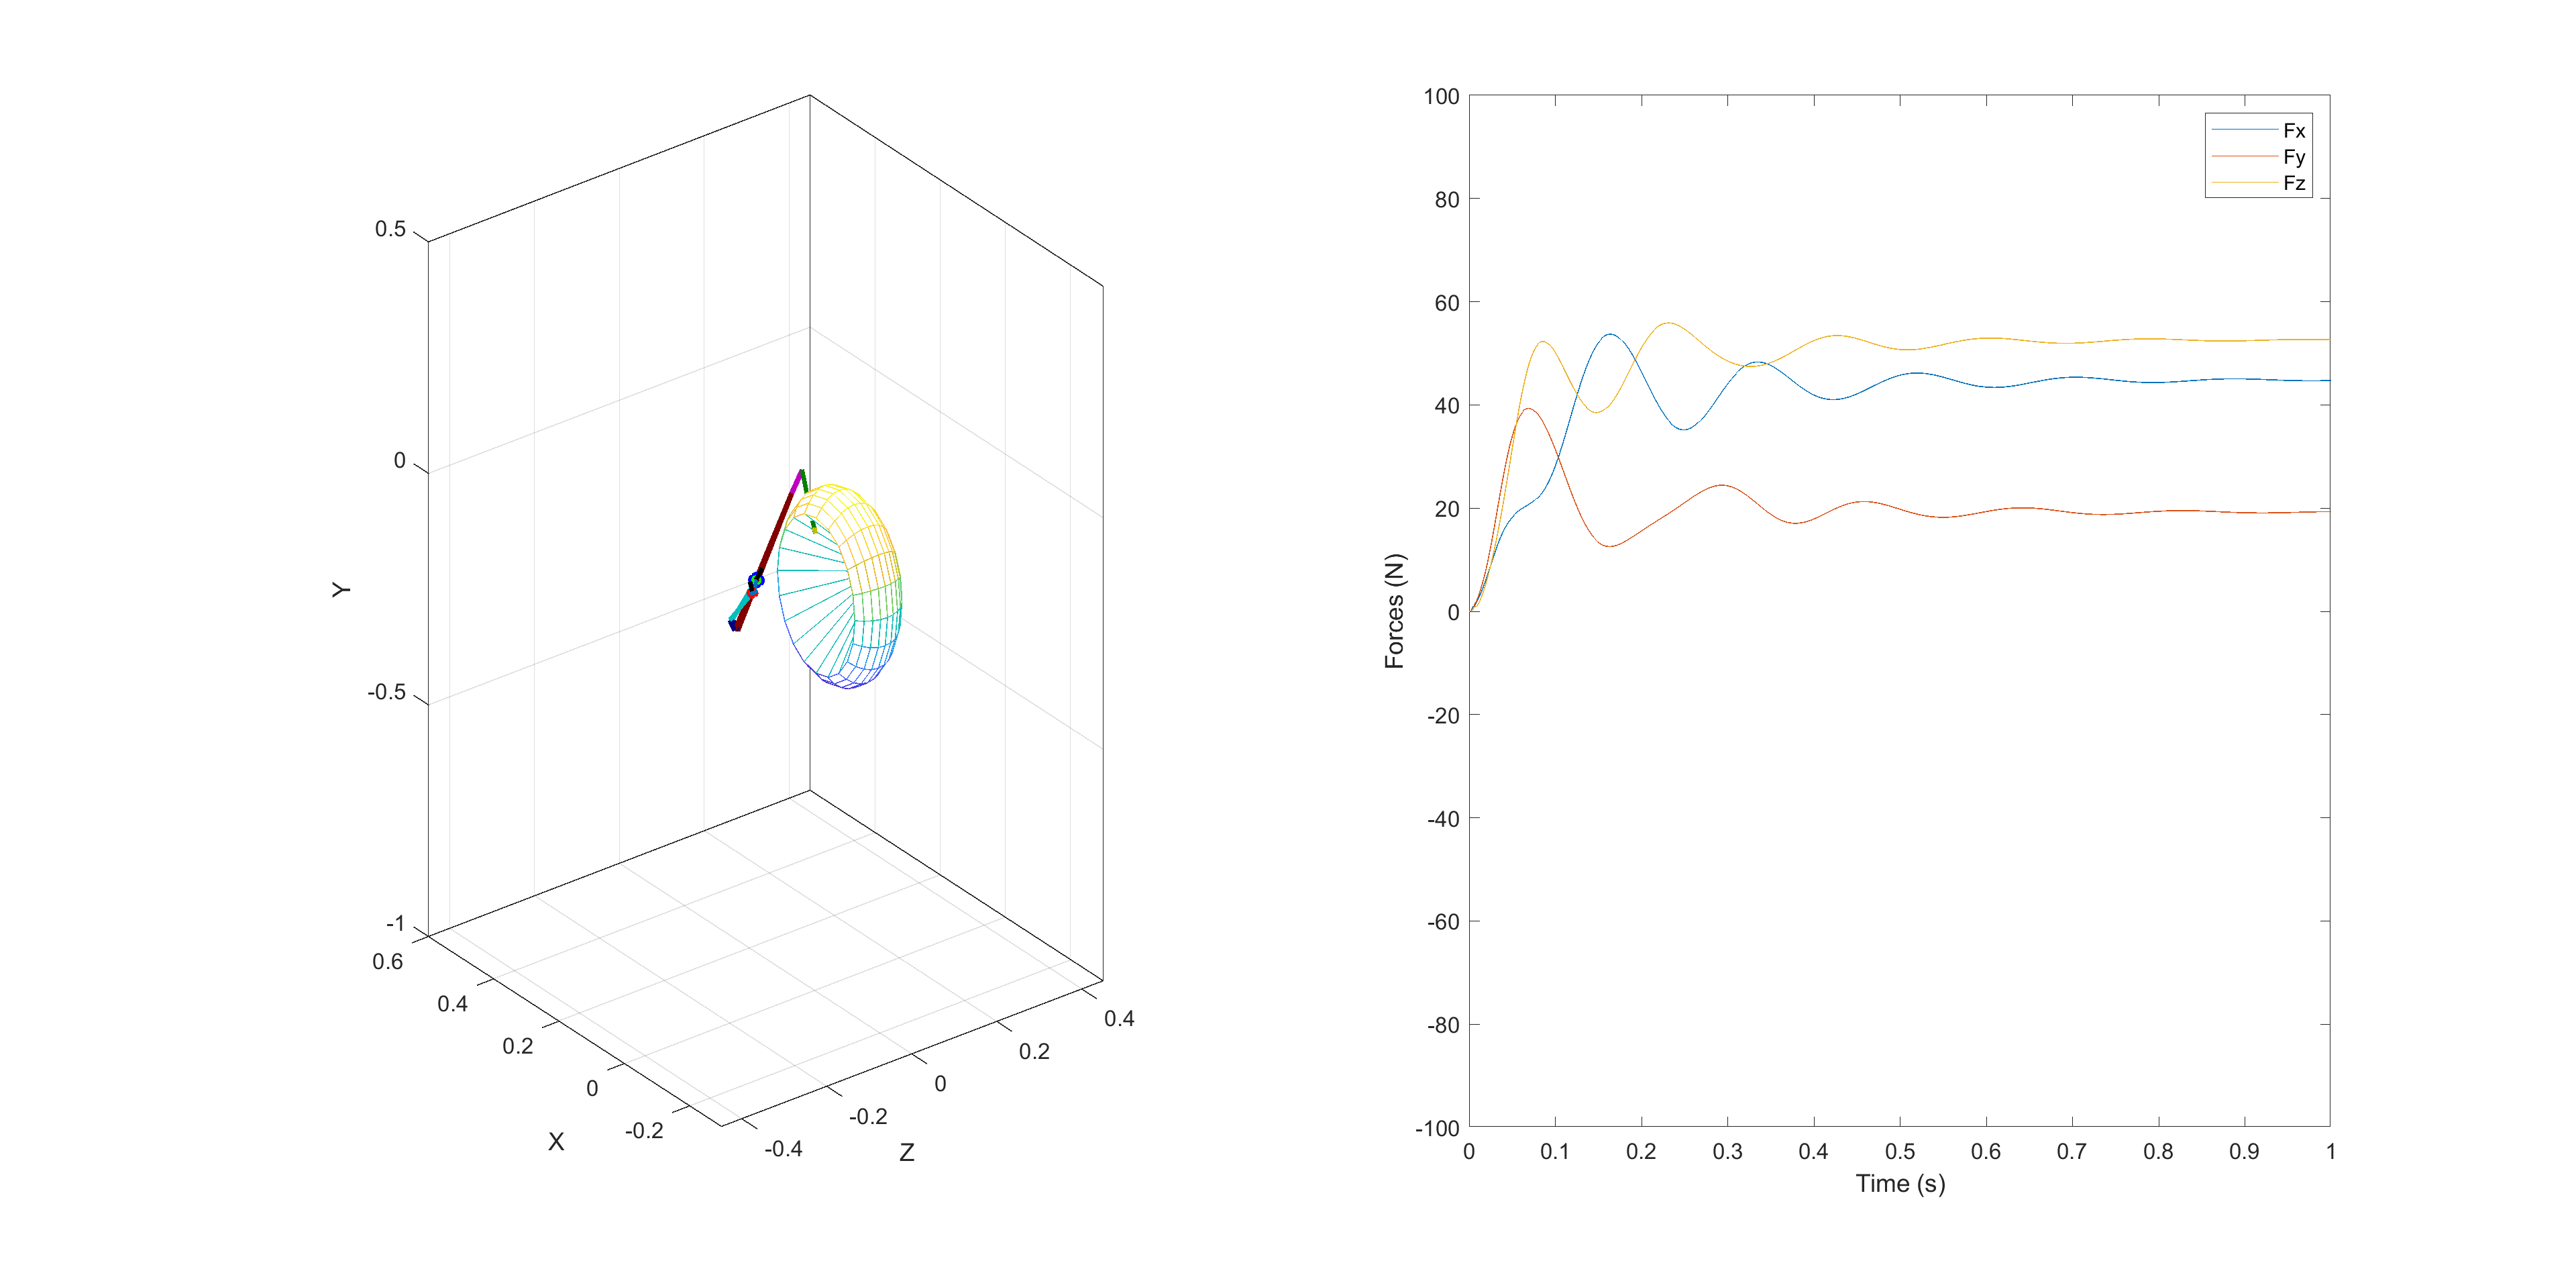
\includegraphics[width=1.1\linewidth]{Pictures/Results/stimuated_1_without_support.png}
        \caption{PI Controller Without Arm Support.}
    \end{subfigure}
    \hfill
    %\vspace{1cm} % Adjust the space between the figures as needed
    \begin{subfigure}[b]{0.45\linewidth}            
        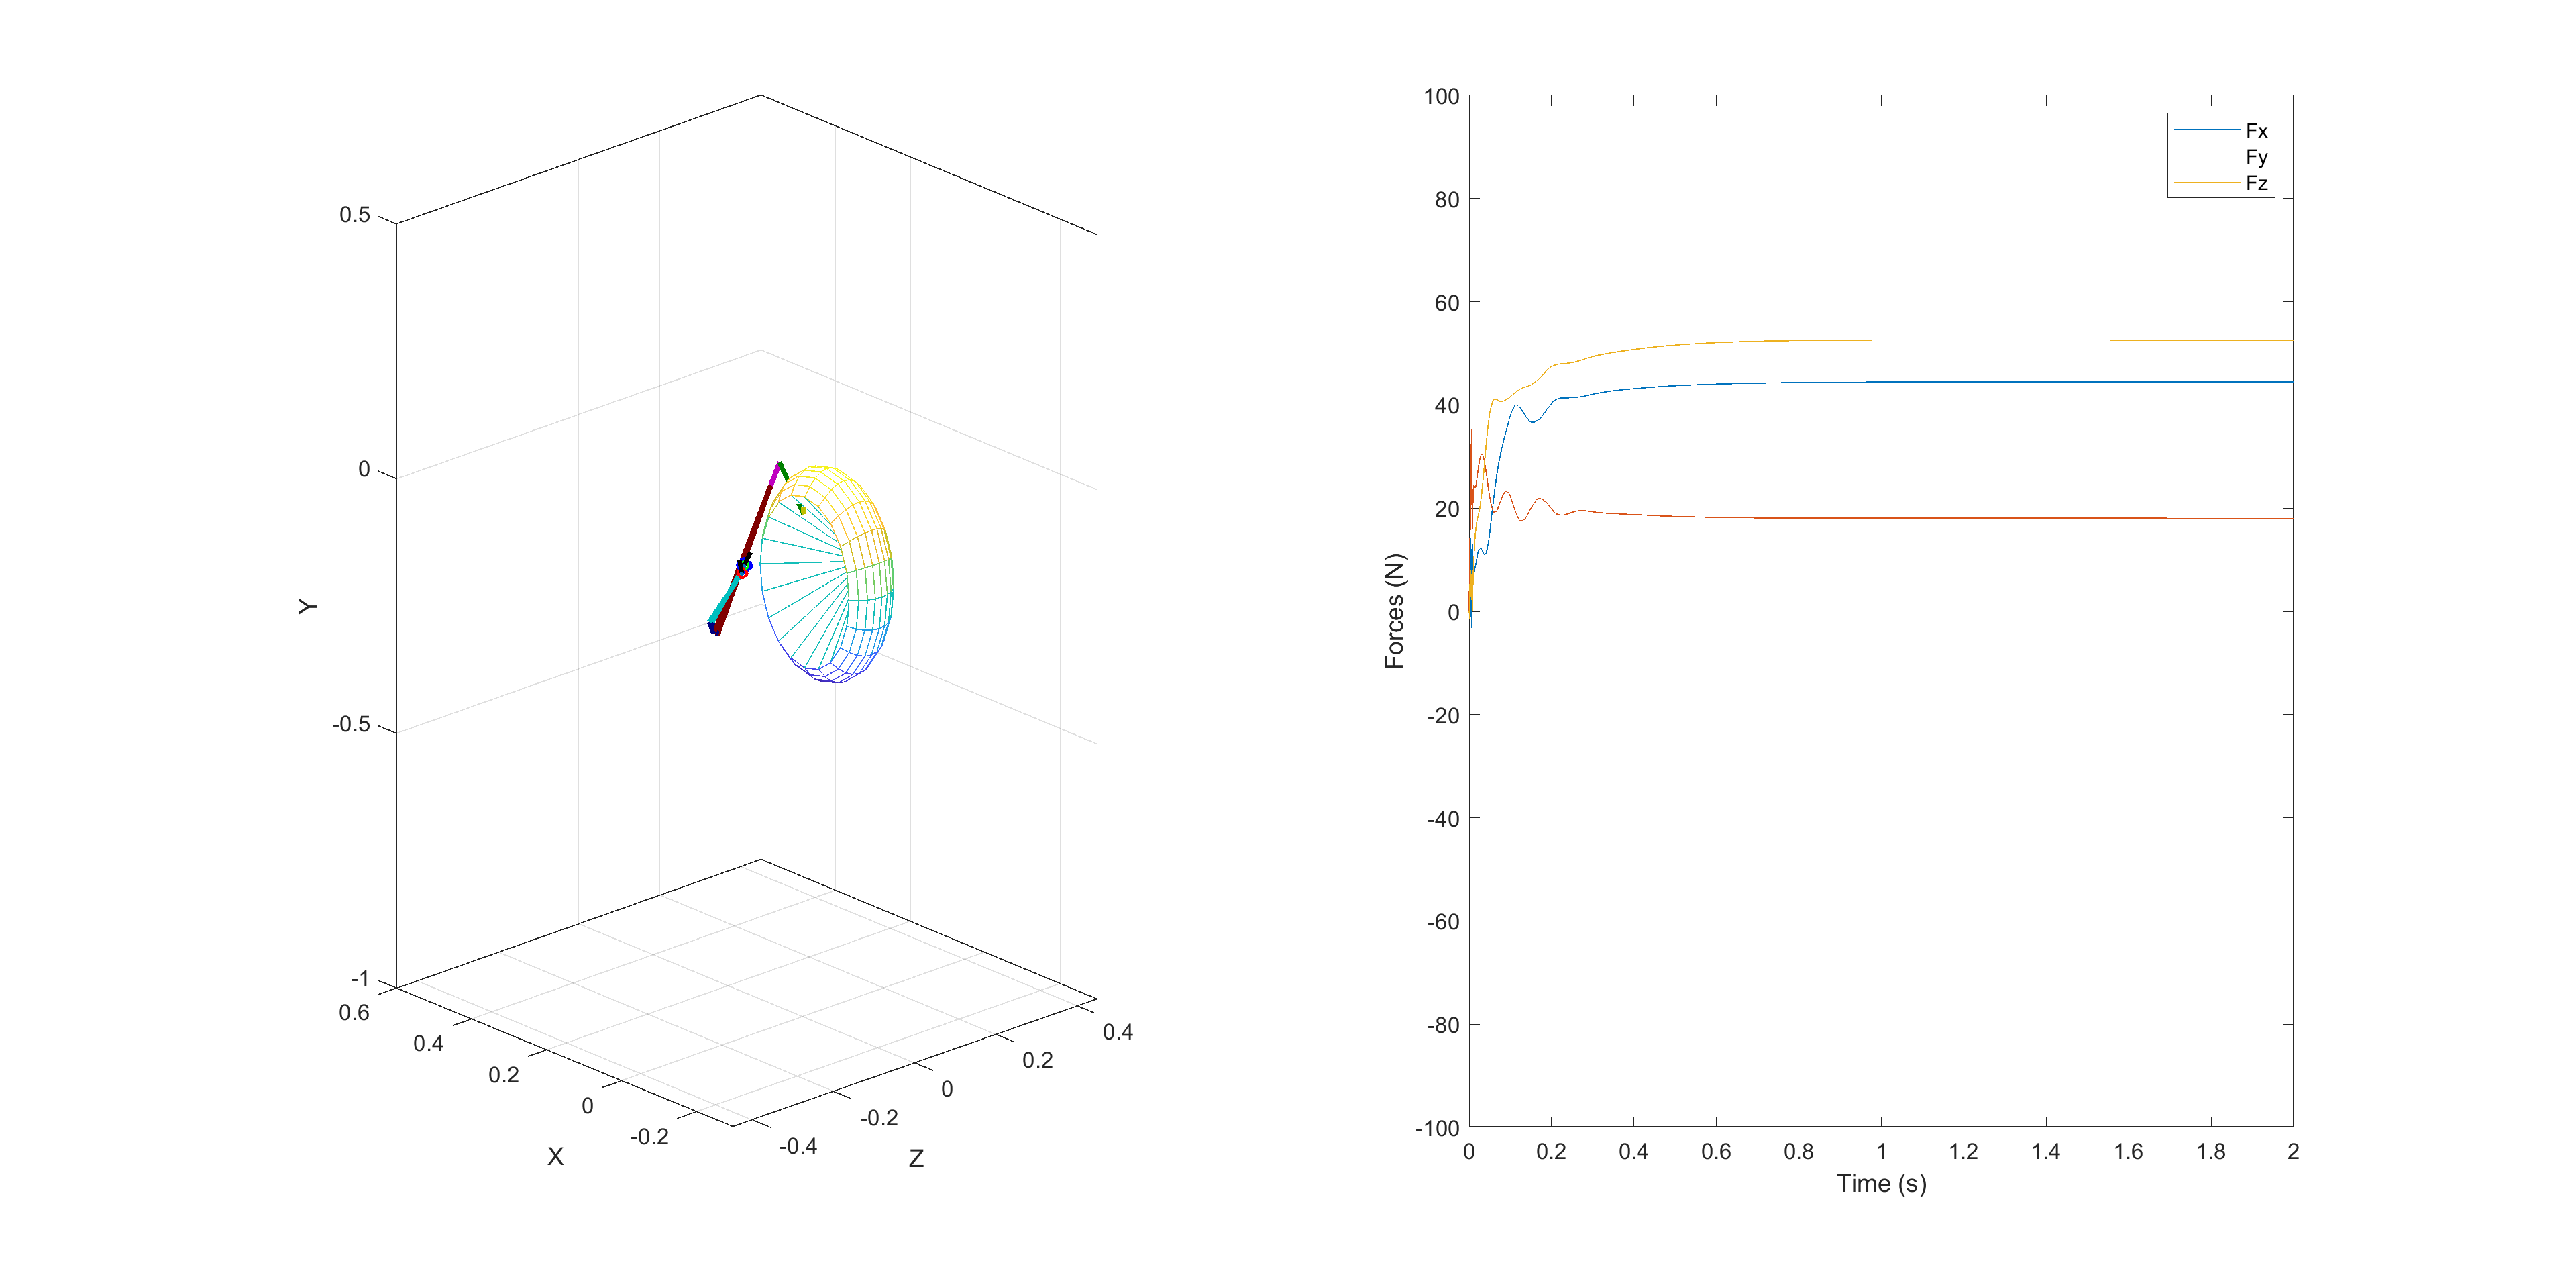
\includegraphics[width=1.1\linewidth]{Pictures/Results/stimuated_1_with_support.png}
        \caption{PI Controller With Arm Support.}
    \end{subfigure}

    \caption{PI Controller for holding Static Position with One Muscle Excitation.}
    \label{fig:PIExcitation}

\end{figure}

\begin{figure}[h!] 
    \centering
    \begin{subfigure}[b]{0.8\linewidth}
       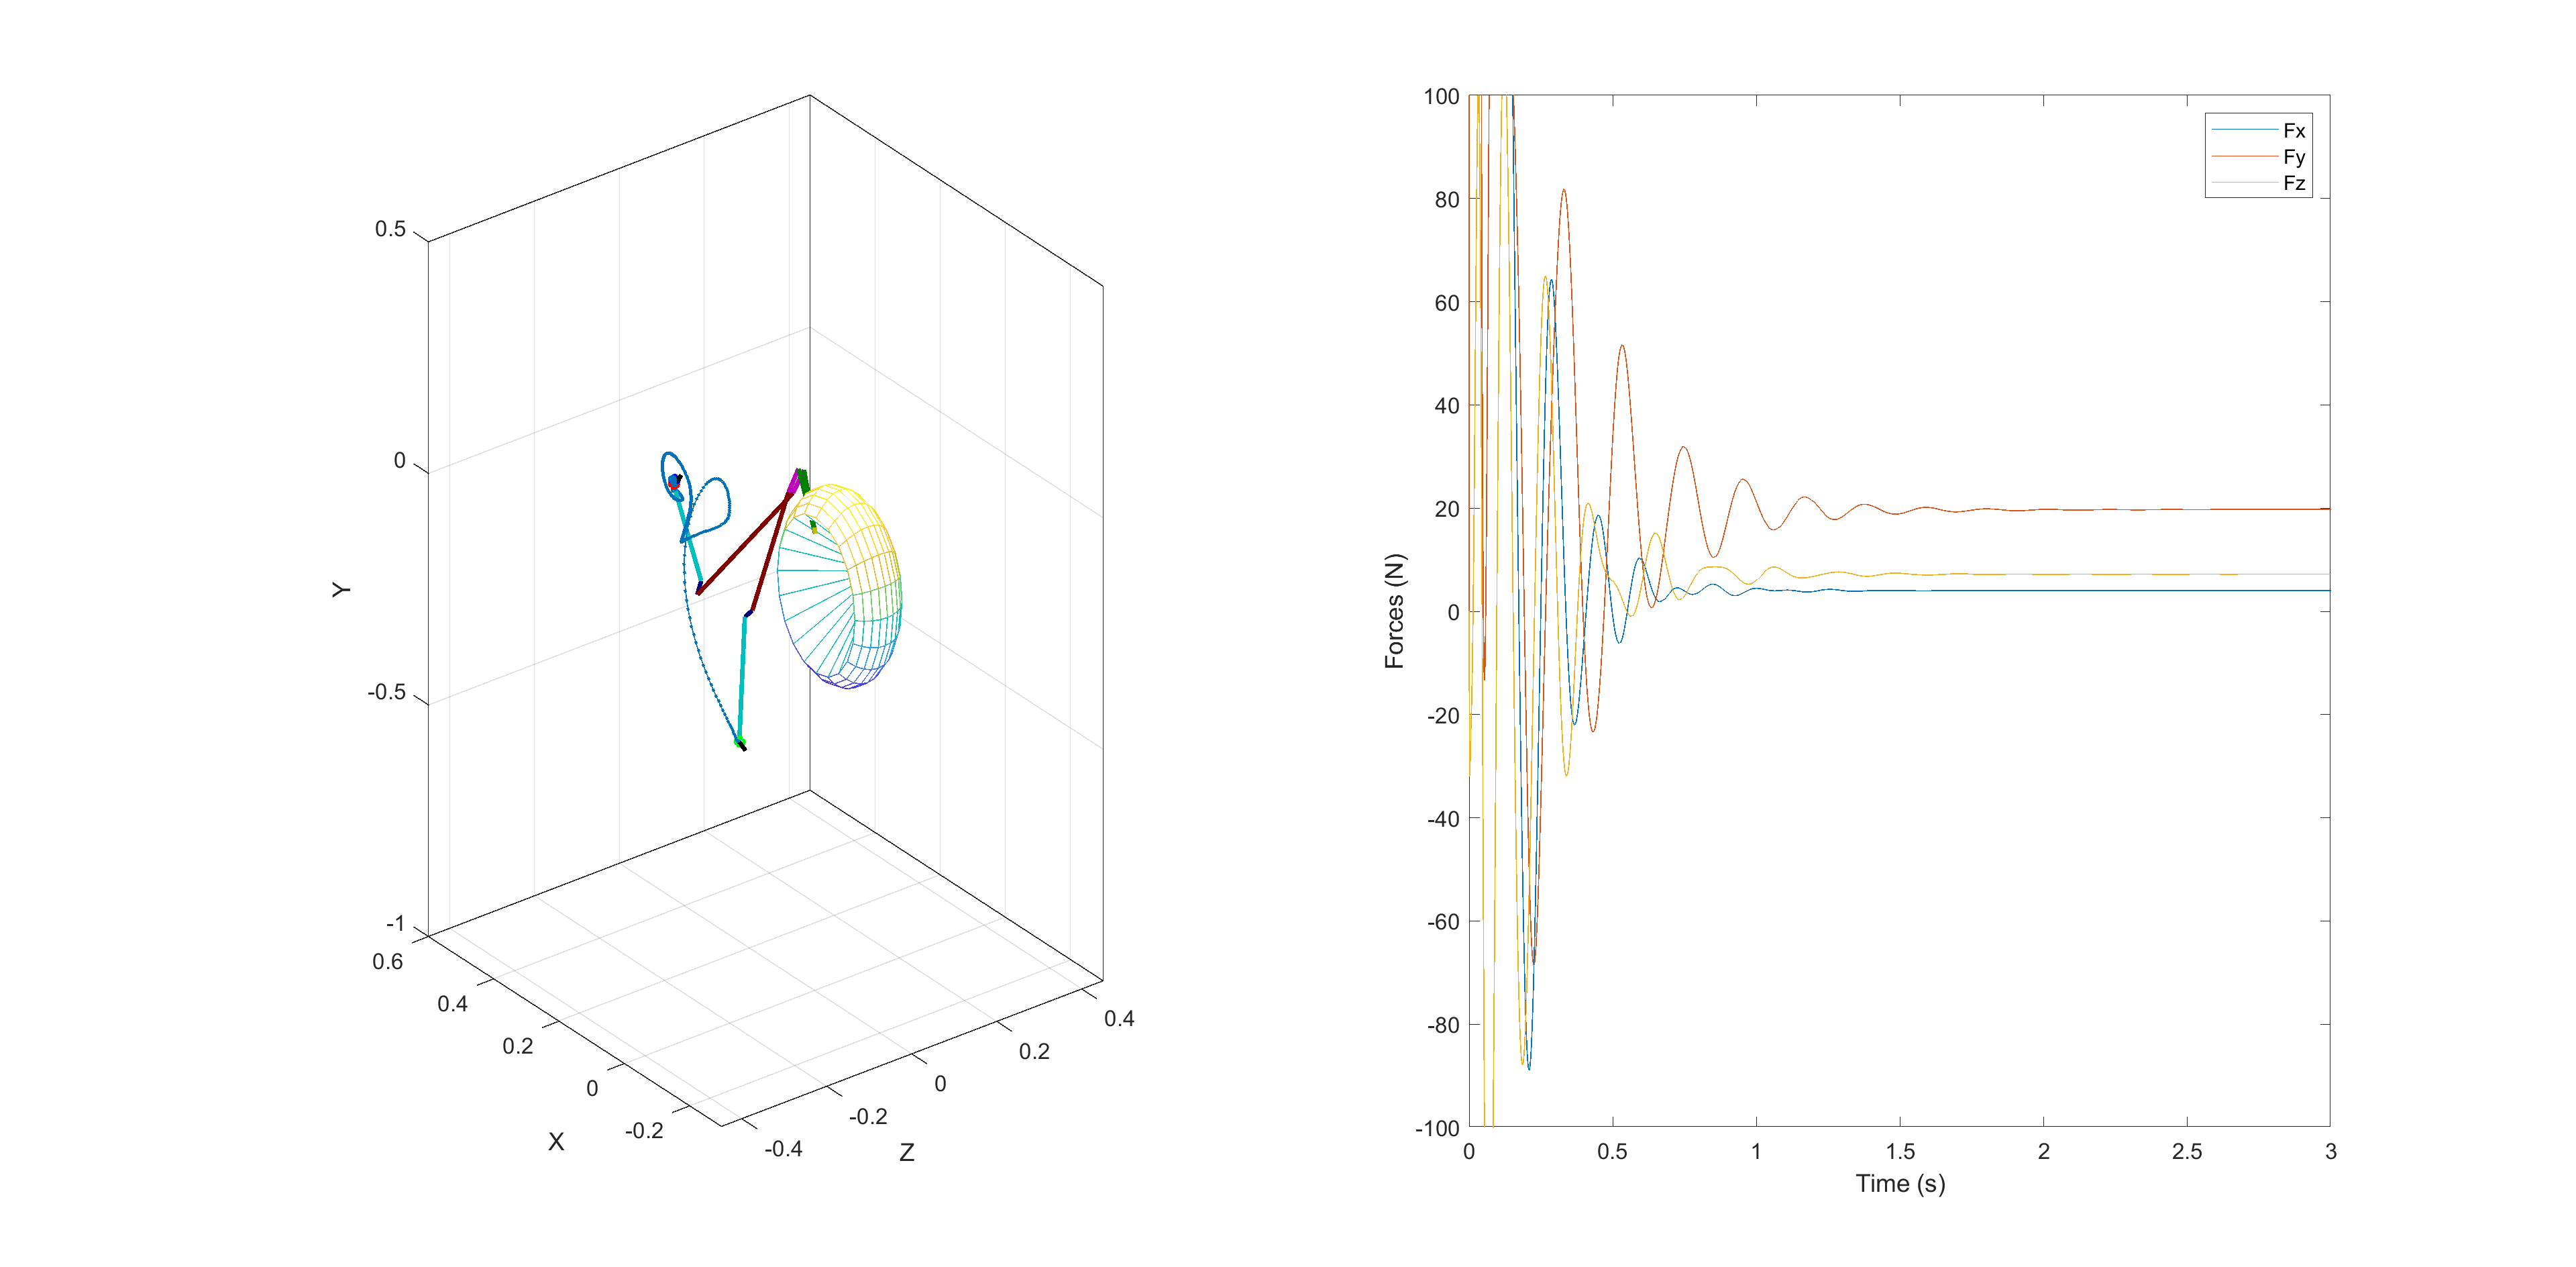
\includegraphics[width=\linewidth]{Pictures/Results/static_without_support.png}
        \caption{PI Controller Without Arm Support.}
    \end{subfigure}

    \vspace{1cm} % Adjust the space between the figures as needed
    \begin{subfigure}[b]{0.8\linewidth}            
        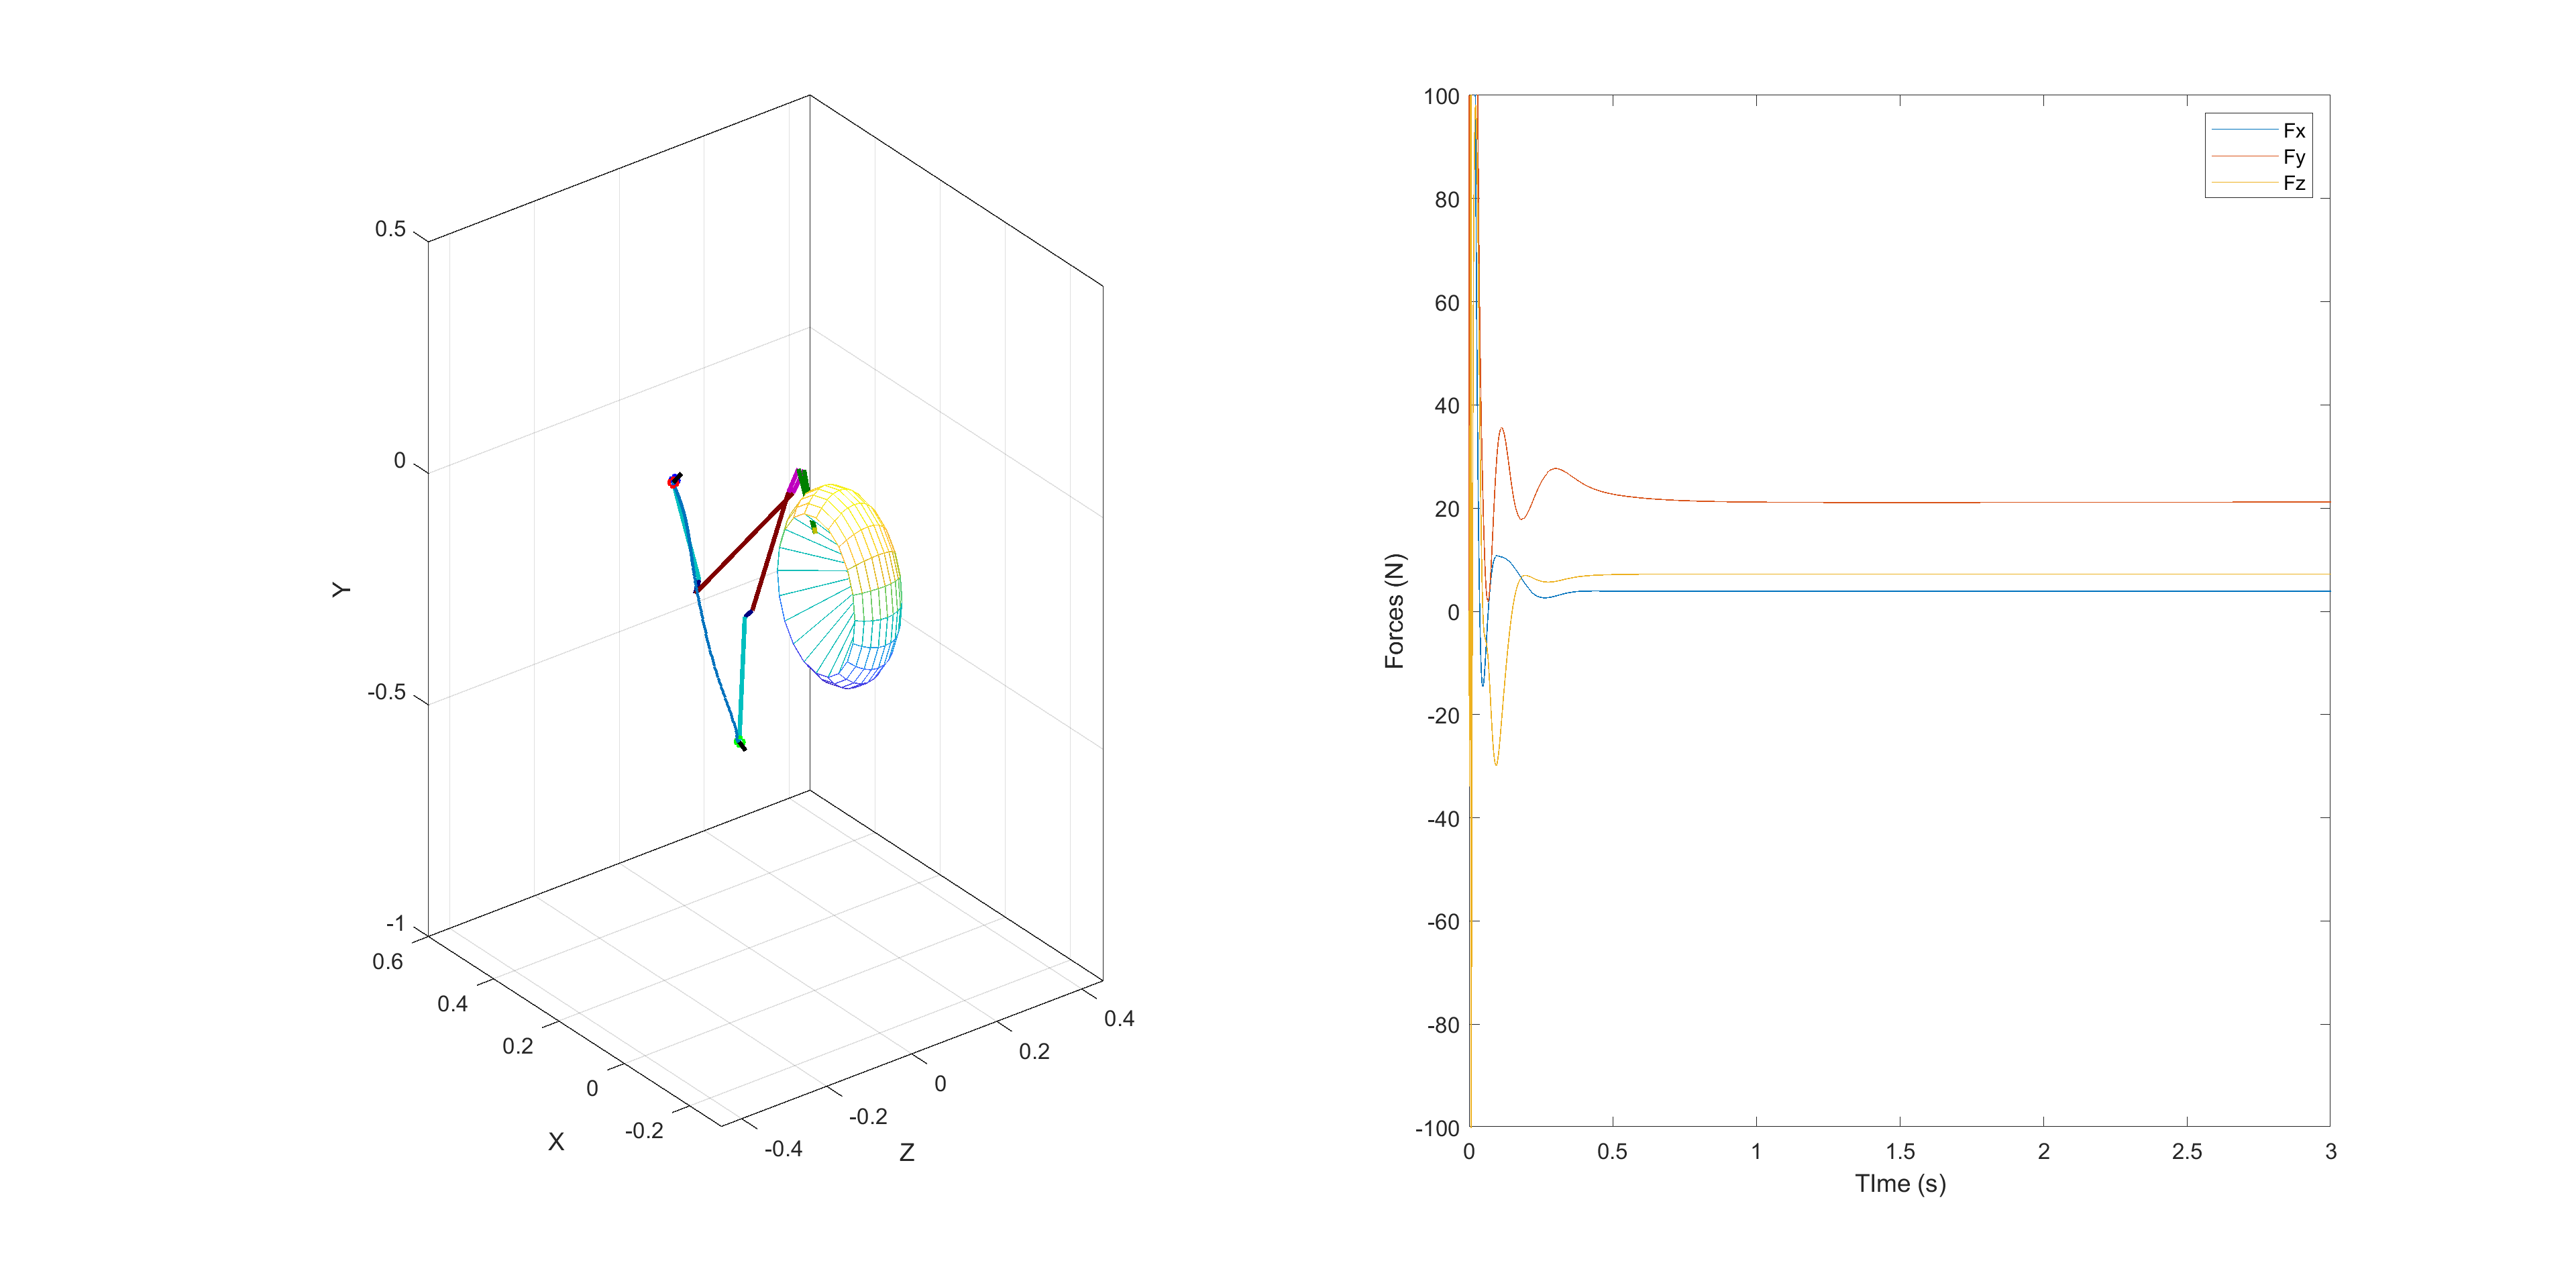
\includegraphics[width=\linewidth]{Pictures/Results/static_with_support.png}
        \caption{PI Controller With Arm Support.}
    \end{subfigure}

    \caption{PI Controller from Equilibrium Position to Static Position with No Muscles Excitation.}
    \label{fig:PINoExcitation}

\end{figure}

